
\chapter{Prompt-Engineering}\label{ch:prompt-engineering}

Im vorherigen Kapitel wurden mehrere \glspl{llm} anhand des entwickelten Benchmarks und einer reduzierten Version der Policy miteinander verglichen.
Auf Grundlage dieser Evaluation wurde \texttt{mistral-small:24b} als Modell zur weiteren Untersuchung und Vertiefung der Forschung ausgewählt.
Die Untersuchung wird in diesem Kapitel auf die vollständige Policy ausgeweitet.
Während im Benchmark ausschließlich die reduzierte Policy mit den Anforderungen \nameref{subsec:cir-01}, \nameref{subsec:cep-01} und \nameref{subsec:cep-02} zur Extraktion verwendet wurde und die Erwartungshaltungen dementsprechend auf diese Teilmenge beschränkt waren, werden im weiteren Verlauf dieser Untersuchung die Erwartungshaltungen so erweitert, dass alle Aspekte berücksichtigt werden, mit Ausnahme der mit \enquote{out of scope} (\nameref{subsec:cir-02}, \nameref{subsec:cep-04}, \nameref{subsec:cep-06}) gekennzeichneten Regeln.
Darauf aufbauend wird durch systematisches Prompt-Engineering eine Optimierung der Extraktionsleistung angestrebt.
Ziel ist es, die Extraktion auf Grundlage der gesamten Policy in einer möglichst hohen Qualität zu ermöglichen.
Die Struktur des Prompts, die Formulierung der Entitätsdefinitionen sowie die Gestaltung der Few-Shot-Beispiele werden dabei schrittweise verfeinert, um die Genauigkeit der Extraktion sukzessive zu erhöhen.

% ======================================================================================================================

\section{Methodisches Vorgehen}\label{sec:methodisches-vorgehen}

Einen methodischen Bezugspunkt bildet die Arbeit von \citeauthor{cheng_novel_2024} \autocite{cheng_novel_2024}, in der ein neuartiges Prompting-Verfahren für Few-Shot \gls{ner} vorgestellt wird.
Das Vorgehen der Autoren basiert auf einer klar strukturierten Gestaltung des Prompts, die mehrere aufeinander abgestimmte Bestandteile umfasst.
Zunächst wird eine Aufgabenbeschreibung formuliert, die das \gls{llm} explizit in die Rolle eines Entity-Recognition-Systems versetzt und die Aufgabe eindeutig umreißt.
Darauf folgt eine präzise Definition der Entitätskategorien, die jeweils mit kurzen Erklärungen versehen werden, um semantische Abgrenzungen zwischen den Klassen deutlich zu machen.
Im nächsten Schritt werden Few-Shot-Beispiele integriert, die als Input-Output-Paare gestaltet sind und sowohl die Extraktion selbst als auch das gewünschte Ausgabeformat illustrieren.
Dieses Ausgabeformat wird zusätzlich separat spezifiziert, sodass das Modell konsistente und strukturierte Ergebnisse erzeugt.
Ergänzend sehen \citeauthor{cheng_novel_2024} \autocite{cheng_novel_2024} die Möglichkeit vor, zusätzliche Instruktionen in den Prompt einzufügen, die wiederkehrende Fehlerquellen adressieren und dadurch die Zuverlässigkeit der Ergebnisse erhöhen \autocite{cheng_novel_2024}.

Zur Optimierung dieses Setups führen die Autoren eine Feedback-Schleife ein.
Das \gls{llm} wird mit dem initialen Prompt auf Trainingsdaten angewandt, die Extraktionen durch das \gls{llm} werden mit den Erwartungshaltungen verglichen und anhand des F1-Scores bewertet.
Anschließend werden die am besten verarbeiteten Beispiele identifiziert und als Demonstrationen in den Prompt übernommen.
Auf diese Weise wird der Prompt iterativ verbessert und stärker auf die spezifischen Anforderungen des Tasks zugeschnitten \autocite{cheng_novel_2024}.

Das Vorgehen in dieser Arbeit orientiert sich in seiner Grundstruktur an der Methodik von \citeauthor{cheng_novel_2024} \autocite{cheng_novel_2024}.
Der Prompt ist ebenfalls in mehrere Komponenten gegliedert, bestehend aus einer Aufgabenbeschreibung, präzisen Entitätsdefinitionen, Beispielen, zusätzlichen Instruktionen sowie einem festgelegten Ausgabeformat.
Die Optimierung wurde iterativ durchgeführt, indem die Definitionen schrittweise angepasst und Beispiele ergänzt wurden, die in vorherigen Versionen zu Fehlern bei der Extraktion geführt hatten.

Ein wesentlicher Unterschied zum Vorgehen von \citeauthor{cheng_novel_2024} \autocite{cheng_novel_2024} besteht darin, dass die Auswahl der Beispiele nicht automatisiert über eine Selektion der besten Beispiele anhand von F1-Scores erfolgte, sondern manuell vorgenommen wurde.
Grundlage dieser Anpassungen war eine gezielte Analyse typischer Fehlerkonstellationen, die sich im Benchmark gezeigt haben.
Diese Vorgehensweise wurde gewählt, da zunächst die Optimierung der Ergebnisse innerhalb des entwickelten Benchmarks im Vordergrund steht, um auf dieser Grundlage die Generalisierbarkeit des Modells auf bislang nicht gesehene Daten zu unterstützen.
Ein vergleichbares Vorgehen kam bereits bei der Erstellung des Benchmark-Prompts zur Anwendung, welcher ebenfalls nach einer Reihe explorativer Experimente manuell angepasst und verfeinert wurde, um die Anforderungen der reduzierten Policy abzubilden.

% ======================================================================================================================

\section{Ergebnisse}

Abbildung~\ref{fig:prompt-engineering-results} zeigt die Resultate des Prompt-Engineerings.
Für die verschiedenen Versionen des Prompts werden zwei Metriken dargestellt.
Einerseits der Prozentsatz der \textit{Exact Matches} und andererseits der \textit{F1-Score}, dessen Werte mit dem Faktor \num{100} multipliziert wurden, um eine direkte Vergleichbarkeit mit den \textit{Exact Matches} zu ermöglichen.
Von Version \texttt{P0} bis \texttt{P7} steigt der Anteil an \textit{Exact Matches} kontinuierlich an, während der \textit{F1-Score} ab Version \texttt{P5} ein Plateau erreicht.
Die Version \texttt{P7.2} erzielt mit \num{96.27} \% den höchsten Wert an \textit{Exact Matches} bei einem \textit{F1-Score} von \num{0.9336}.

\begin{figure}[ht]
    \centering
    \makebox[\textwidth]{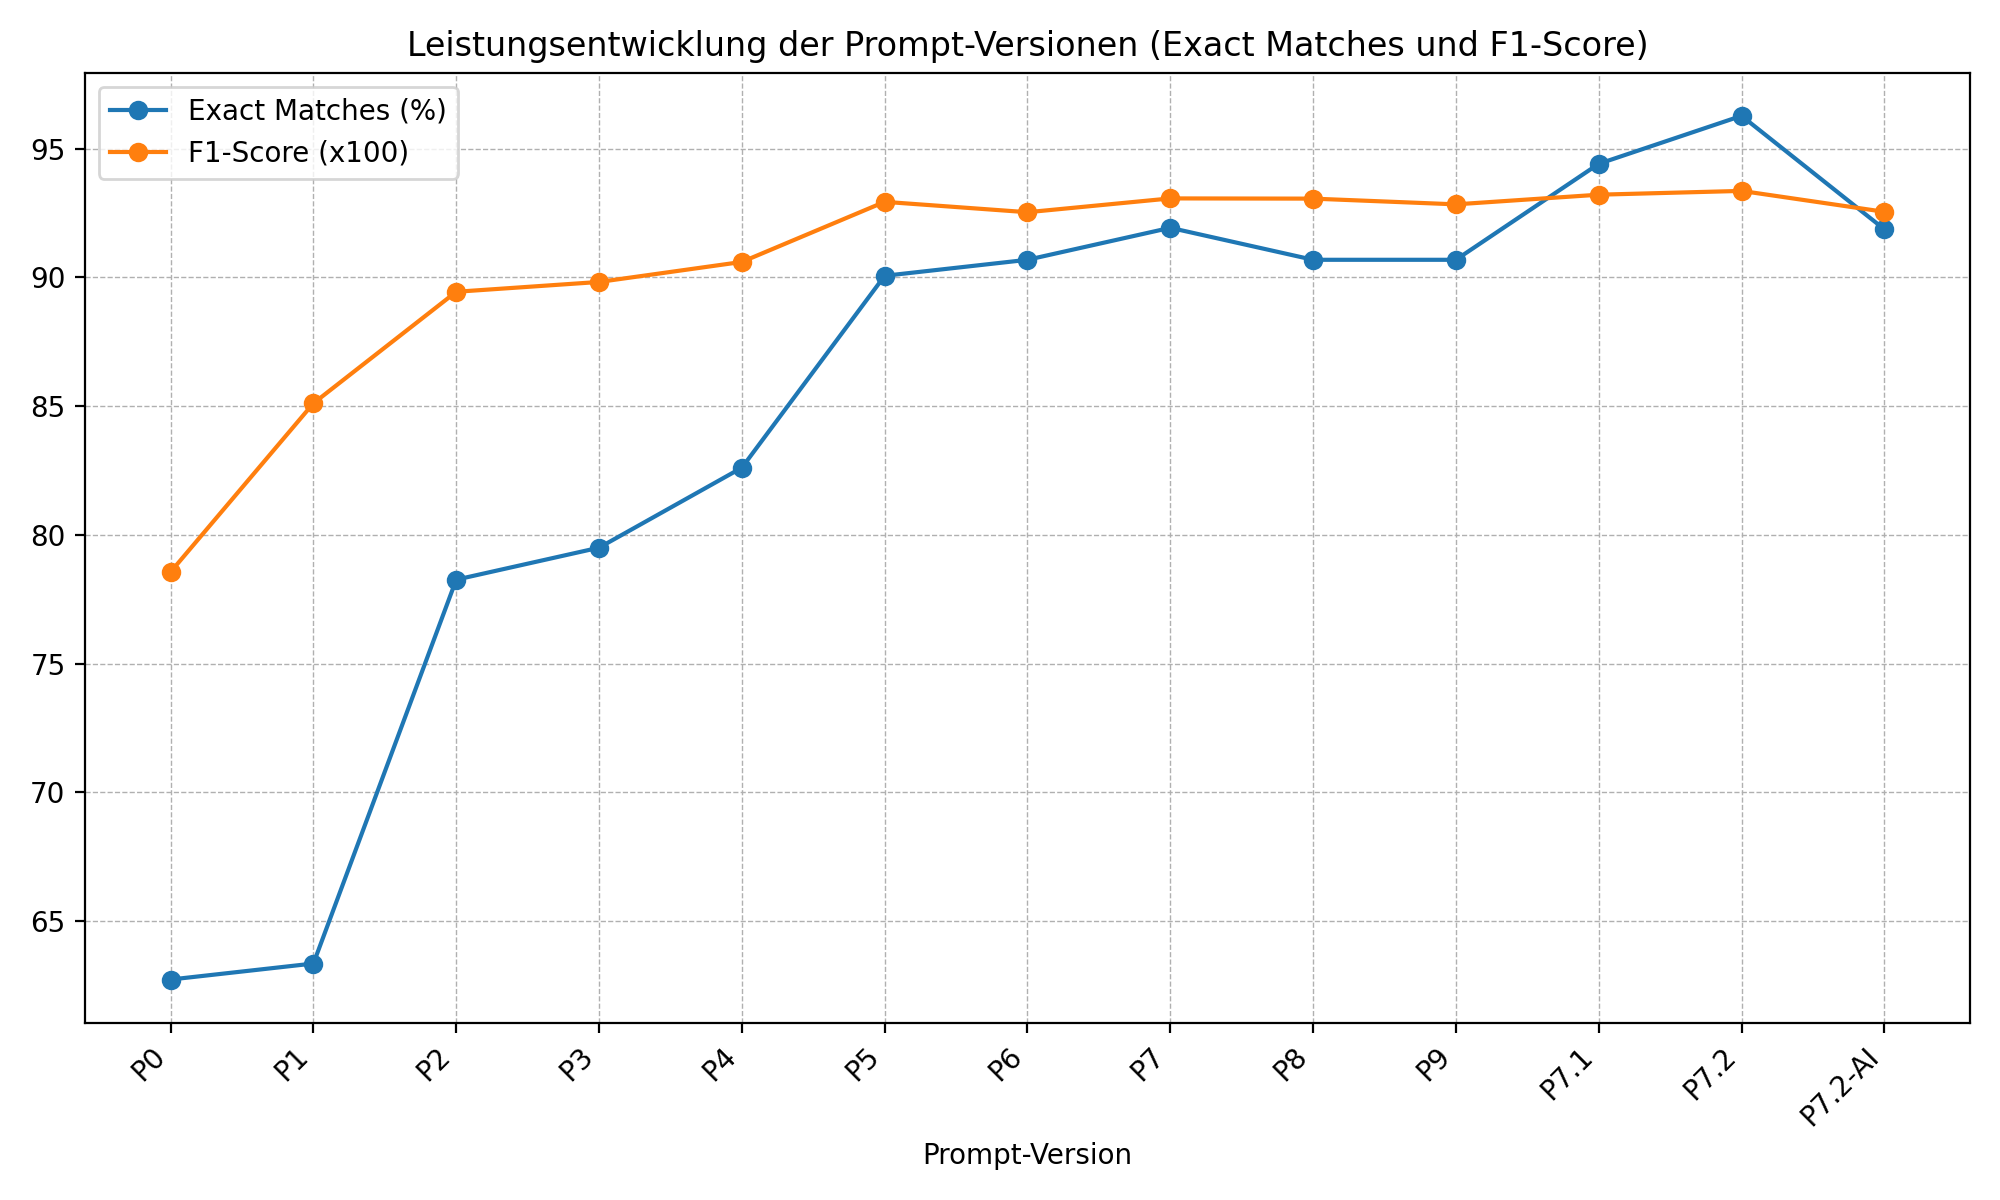
\includegraphics[width=1.3\textwidth]{prompt-engineering/prompt_versions_performance.png}}
    \caption{Entwicklung der Extraktionsleistung über die verschiedenen Prompt-Versionen. Dargestellt sind die Exact Matches und die F1-Scores (multipliziert mit 100). Die Werte steigen bis Version P7 kontinuierlich an, wobei die Version P7.2 die besten Ergebnisse erzielt.}
    \label{fig:prompt-engineering-results}
\end{figure}

Der Prompt \texttt{P0} stellt den Ausgangspunkt dar, mit dem der Benchmark durchgeführt wurde.
Erwartungsgemäß erreicht diese Version mit \num{62.73} \% einen niedrigen Wert bei den \textit{Exact Matches}, da sie ausschließlich auf der reduzierten Policy basierte.
In den Versionen \texttt{P1} bis \texttt{P9} wurden die Entitätsdefinitionen sukzessive erweitert, sodass die zusätzlichen Aspekte der vollständigen Policy berücksichtigt wurden.
In \texttt{P1} wurden zunächst Erklärungen aufgenommen, die den Anforderungen \nameref{subsec:cep-03}, \nameref{subsec:gep-01} und \nameref{subsec:air-01} entsprechen.
Mit \texttt{P2} kamen Definitionen für die \nameref{subsec:aep-01} und die \nameref{subsec:hep-01} hinzu.
Zusätzlich wurden Beispiele konstruiert, die \textit{Authors} und \textit{Holders} mit E-Mail-Adressen beinhalten und damit \nameref{subsec:gep-01} abbilden, sowie Beispiele, die Blöcke von Copyright-Statements enthalten und damit \nameref{subsec:cep-03} berücksichtigen.
Dabei wurde sichergestellt, dass die Beispiele keine Inhalte umfassen, die Teil des Benchmarks sind, um Überschneidungen zwischen Trainings- und Testdaten zu vermeiden.

In \texttt{P3} wurden weitere Beispiele ergänzt.
Da das \gls{llm} Schwierigkeiten bei der korrekten Erkennung von Blockstrukturen mit mehreren Copyrights zeigte, wurde in \texttt{P4} die Definition dieser Struktur präzisiert.
Mit \texttt{P5} wurde ein Beispiel für einen umfangreichen Block mit sechs Copyright-Statements hinzugefügt sowie ein Beispiel, das irrelevante Lizenzhinweise enthält, die bei der Extraktion nicht übernommen werden sollten.

Die Versionen \texttt{P7} bis \texttt{P9} wurden vor allem durch zusätzliche Beispiele erweitert.
Während der Anteil an \textit{Exact Matches} in \texttt{P7} den höchsten Wert dieser Serie erreichte, sank er in den nachfolgenden Versionen wieder leicht ab.
Daher wurde die Version \texttt{P7} erneut aufgegriffen und als Grundlage für weitere Optimierungen genutzt.
Diese Erweiterungen erfolgten durch zusätzliche Instruktionen nach den Few-Shot-Beispielen, wie sie auch von \citeauthor{cheng_novel_2024}\ empfohlen werden \autocite{cheng_novel_2024}.

In den Versionen \texttt{P7.1} und \texttt{P7.2} wurden ergänzende Erklärungen integriert, die klarstellen, dass Lizenzinformationen nicht Teil der Copyrights sind und dass Kommentarsyntax vor und nach den Statements zu vermeiden ist.
Außerdem wurde ein weiteres Beispiel aufgenommen, das die korrekte Extraktion von Statements in Ascii-Art verdeutlicht.
Die Version \texttt{P7.2} enthält insgesamt sieben Few-Shot-Beispiele und wird für die nachfolgenden Untersuchungen verwendet.
Der vollständige Prompt ist im Anhang~\ref{sec:anahng-prompt-p7.2} aufgeführt.

Im Anschluss wurde ein Experiment mit GPT-5 \footnote{\url{https://openai.com/index/introducing-gpt-5/}} durchgeführt, bei dem das Modell aufgefordert wurde, den Prompt \texttt{P7.2} zu optimieren.
Der resultierende Prompt ist als \texttt{P7.2-AI} in den Ergebnissen gekennzeichnet und im Anhang~\ref{sec:anahng-prompt-p7.2-ai} hinterlegt.
Die wesentliche Änderung bestand darin, dass die Beschreibungen der Entitäten in eine stichpunktartige Struktur umgewandelt und sprachlich leicht angepasst wurden.
Die Ergebnisse zeigen jedoch, dass diese Anpassung einen geringeren Anteil an \textit{Exact Matches} von \num{91.86} \% zur Folge hatte.

% ======================================================================================================================

\section{Validierung mit ungesehenen Daten}

Nachdem im Rahmen des Benchmarks eine Optimierung des Eingabeprompts durchgeführt wurde, erfolgte im nächsten Schritt eine Validierung mit bisher ungesehenen Daten.
Zu diesem Zweck wurde ein Datensatz zusammengestellt, der aus \num{200} Dateien der Kategorie \enquote{single copyrights without authors} sowie \num{200} Dateien der Kategorie \enquote{multiple copyrights with authors} besteht.
Für alle Dateien wurden die Erwartungshaltungen gemäß der vollständigen Policy definiert.
Bei der Kuratierung wurde darauf geachtet, dass jedes Copyright-Statement nur einmal im Datensatz vorkommt, um Wiederholungen zu vermeiden.

Die Extraktion der \enquote{single copyrights without authors} erreichte einen Wert von \num{99} \% \textit{Exact Matches}, was auf eine sehr gute Generalisierungsfähigkeit der optimierten Lösung in diesem einfachen Szenario hinweist.
Im Fall der \enquote{multiple copyrights with authors} lag der Anteil an \textit{Exact Matches} hingegen lediglich bei \num{73.88} \%.
Dieses Ergebnis verdeutlicht, dass die Optimierung zwar für einfache Extraktionsaufgaben eine robuste Leistung erzielt, bei komplexeren Strukturen mit mehreren Statements und Autoren jedoch noch deutliche Einschränkungen bestehen.

% ======================================================================================================================

\section{Analyse der ScanCode False-Negatives}

Da der Vergleich zwischen dem ScanCode-Toolkit und der \gls{llm}-basierten Lösung einen zentralen Bestandteil dieser Arbeit darstellt, wurde ein isoliertes Experiment durchgeführt.
Aus der Kategorie \enquote{no copyrights or authors or holders} des Datensatzes wurden \num{3000} Dateien zufällig ausgewählt und auf das Vorkommen von Copyright-Statements untersucht.
Diese Kategorie umfasst Dateien, in denen das ScanCode-Toolkit keine Copyright-Informationen identifizieren konnte.
Ziel der Analyse war daher zu prüfen, ob die optimierte \gls{llm}-Lösung in diesen Fällen dennoch Copyright-Statements extrahieren kann, die als False-Negatives des ScanCode-Toolkits zu interpretieren sind.

Die Untersuchung ergab, dass die optimierte \gls{llm}-Lösung insgesamt \num{20} Copyright-Statements extrahieren konnte.
Der Großteil dieser Funde stammt aus Binärdateien, was darauf hindeutet, dass das \gls{llm} im Gegensatz zum regelbasierten Ansatz des ScanCode-Toolkits in der Lage ist, auch in diesem Dateityp relevante Informationen zu erkennen.

Darüber hinaus wurde ein weiterer Fall entdeckt, bei dem ein Copyright-Statement in einer HTML-Datei durch das ScanCode-Toolkit nicht erkannt wurde:

\begin{lstlisting}[keepspaces=true]
[...]
REVISION
</b><br>
<P>
Last updated: 12 October 2023
<br>
Copyright &copy; 1997-2023 University of Cambridge.
<br>
<p>
Return to the <a href="index.html">PCRE2 index page</a>.
</p>
\end{lstlisting}

Die \gls{llm}-Lösung extrahierte hierbei folgende Informationen:

\begin{lstlisting}[keepspaces=true]
{
    "copyrights": ["Copyright &copy; 1997-2023 University of Cambridge."],
    "holders": ["University of Cambridge"],
    "authors": ["Philip Hazel"]
}
\end{lstlisting}

Dies ist ein Anzeichen dafür, dass es eventuell weitere Strukturen von Copyright-Statements gibt, die das ScanCode Toolkit derzeit nicht erkennt, welche aber durch das semantische Verständnis des \gls{llm} korrekt identifiziert werden können.
Eine tiefgreifendere Analyse der False-Positives könnte weitere solcher Fälle aufzeigen und zur Erweiterung des Testdatensatzes besonders relevant sein.
Weiterhin könnte dieser Ansatz der gegenläufigen Prüfung auch bei anderen Datenkategorien zur Identifikation besonderer Fälle und zur weiteren Schärfung der Policy genutzt werden.